\documentclass[a4paper,12pt]{article}
\usepackage{titlesec}
\usepackage{xcolor}
\usepackage{listings}
\usepackage{a4wide}                          
\usepackage{lipsum}
\usepackage{amsmath}                       
\usepackage{amsfonts}                      
\usepackage[pdftex]{graphicx}               
\usepackage{sidecap}                      
\usepackage{floatrow}        
\usepackage{subfig}            
\usepackage{fontawesome}
\usepackage[version=4]{mhchem}       
\usepackage{mathtools}
\usepackage{float}
\usepackage{flafter}
\usepackage[section]{placeins}
\usepackage{sidecap}                
\usepackage{floatrow} 
\usepackage{subfig}
\usepackage[framemethod=default]{mdframed}
\usepackage{capt-of}  
\usepackage{mhchem}
\usepackage[utf8]{inputenc}
\usepackage{graphicx}
\usepackage{fontenc}
\usepackage{mhchem}
\usepackage{siunitx}
\usepackage{tikz}
\usepackage{xcolor}
\usepackage{listings}
\usepackage{blindtext}
\usepackage[utf8]{inputenc}
\usepackage[english]{babel}
\usepackage{geometry}
\usepackage{fancyhdr}
\usepackage{xcolor}
\usepackage{amsmath}
\usepackage{fancyhdr}
\usepackage{xurl}
\usepackage{subfig}
\usepackage{listings}



 \geometry{
 a4paper,
 total={170mm,257mm},
 left=25mm,
 right=25mm,
 bottom=20mm,
 top=20mm,
 }


\floatsetup[table]{capposition=top}

\renewcommand{\tablename}{Table} 


\title{\vspace{0cm}{\sc Project 1: Regression analysis and resampling methods \\ {\large FYS-STK4155 — Applied data analysis and machine learning }}}




\author{Jamal Sharifi  \\ \url{https://github.com/Jamshar} }



\setcounter{page}{0}
\cleardoublepage
\pagestyle{fancy}
\fancyhf{}
\rhead{Project 1 }
\lhead{FYS-STK4155}
\rfoot{Page \thepage }





\begin{document}



\renewcommand{\figurename}{Fig.} 

\onecolumn

\maketitle

\begin{abstract}
\noindent
This project compares ordinary least squares, Ridge and LASSO regression algorithms in order to fit simulated data generated from Franke’s function and to fit real geographical data. Resampling techniques were used to estimate confidence intervals, bias-variance decomposition and assessing performance of predictive models, in order to identifying optimal parameters such as polynomial degree and penalty parameter $\lambda$. Ordinary least squares performed well with data of moderate size and low model complexity. For both simulated and real-world geographical data ordinary least squares was outperformed by Ridge and LASSO when dealing with overfitting.


\end{abstract}



\thispagestyle{empty}
\tableofcontents 




\section{Introduction}
Statistics and machine learning are closely related and are important tools for solving real-world problems using different algorithms. The algorithms are developed to learn and make predictions from data as well as extract statistical quantities in the data. Through linear regression one aims to find the relationship between the target variable and the features in the data by finding models that describes the data and allows for predictions of the target variable based on the features in the data.The advantages of linear regression are many, this includes its simplicity to understand and implement at the same time you have a prior knowledge that there exists an analytical solution to the problem. It has a broad applicability across diverse real-world problems through various scientific disciplines.\\

\noindent
The aim of this project is to explore and compare models using ordinary least squares, Ridge and LASSO regression to be fitted with polynomial features to two sets of three-dimensional datasets. First, the regression methods are implemented to study the Franke’s function and then applied to terrain data, where the elevations is the target variable we want to predict given the geographic positions. After the methods are implemented, the model’s performance and accuracy is then assessed using resampling techniques bootstrapping and k-fold cross validation.\\

\noindent
This report is structured into 5 chapters. Chapter 2 provides an overview of the theory of the linear regression methods, statistical estimations, model assessment, and the resampling techniques employed in the analysis, along with implementations of the methods. In chapter 3, the data sets used in this project are introduced. Chapter 4 is dedicated to presenting the results, and finally, chapter 5 offers the conclusions drawn from the analysis.\\



\section{Theory and Methods}
\subsection{Preprocessing}
The cost function used in this project is the sum of squared residuals,


\begin{equation} \label{eq1}
\begin{split}
C(\boldsymbol{X},\boldsymbol{\beta}) &=\frac{1}{n}\sum_{i=0}^{n-1}(y_i-\tilde{y}_i)^2\\
&=\mathbb{E}\left[(\boldsymbol{y}-\boldsymbol{\tilde{y}})^2\right] \\
&=\frac{1}{n} (\boldsymbol{y-\tilde{y}})^{\boldsymbol{T}} (\boldsymbol{y-\tilde{y}}),
\end{split}
\end{equation}
where the domain of the dataset is $\mathbf{X}_\mathcal{D}=\{(y_j, \boldsymbol{x}_j), j=0\ldots n-1\}$.\\

\noindent
The R-squared score is used for evaluating the quality of fits,
\begin{equation} \label{eq1}
\begin{split}
R^2 &=1-\frac{\sum_{i=0}^{n-1}(y_i-\tilde{y}_i)^2}{\sum_{i=0}^{n-1}(y_i-\bar{y})^2},
\end{split}
\end{equation}
\noindent
where
\begin{equation} \label{eq1}
\begin{split}
\bar{y} &=\frac{1}{n}\sum_{i=0}^{n-1}y_i
\end{split}
\end{equation}

\noindent
This project involves the construction of feature matrices for three-dimensional data, which consist of features structured as follows

\begin{equation} \label{}
\begin{split}
\boldsymbol{X}=[x_1,x_2,x_1^2,x_1x_2,x_2^2, \dots]^T
\end{split}
\end{equation}

\noindent
I have excluded the intercept term since in some cases it has negative effects on the mean squared error. The feature matrix  involves $d=\frac{1}{2}(p+1)\cdot(p+2)-1$ features and  coefficients to be determined. After optimal $\boldsymbol{\tilde{\beta}}$ values have been found, the $\tilde{\beta_0}$  is retrieved using the following expression,
\begin{equation} \label{}
\begin{split}
\tilde{\beta_0}=\frac{1}{n} \sum_{i=0}^{d-1}\text{ytrain}_i - \frac{1}{n}\sum_{i=0}^{d-1}\mathbf{X_i}\cdot \, \boldsymbol{\tilde{\beta_i}} 
\end{split}
\end{equation}

\noindent 
where ytrain is the dependent variable in the training set. I have throughout this project used 80 \% of the data for training and 20 \% for testing. \\

\noindent 
For all of the various models tested I have mean centered the features in the feature matrix as it haas improved model performance. The terrain data was min-max scaled and the altitudes was scaled to match the Franke's function for comparability.
\begin{equation} \label{}
\begin{split}
X=\frac{X-X_{\text{min}}}{X_{\text{max}}-X_{\text{min}}} 
\end{split}
\end{equation}





\subsection{Ordinary Least Squares}
Using the Mean Squared Error (MSE) as the cost function, gives the following optimization problem,

\begin{equation} \label{eq1}
\begin{split}
{\displaystyle \min_{\boldsymbol{\beta}\in {\mathbb{R}}^{p}}}\frac{1}{n}\left\{\left(\boldsymbol{y}-\boldsymbol{X}\boldsymbol{\beta}\right)^T\left(\boldsymbol{y}-\boldsymbol{X}\boldsymbol{\beta}\right)\right\}.
\end{split}
\end{equation}

 \noindent
And when expanding, we get the following cost function,
\begin{equation} \label{eq1}
\begin{split}
C[\boldsymbol{\hat{\beta}}]&=\frac{1}{n}(\boldsymbol{y}-\boldsymbol{X}\hat{\boldsymbol{\beta}})^T(\boldsymbol{y}-\boldsymbol{X}\hat{\boldsymbol{\beta}})\\
&=\frac{1}{n}[\boldsymbol{y}^T\boldsymbol{y}-\boldsymbol{y}^T\boldsymbol{X}\hat{\boldsymbol{\beta}}-(\boldsymbol{X}\hat{\boldsymbol{\beta}})^T\boldsymbol{y}+(X\hat{\boldsymbol{\beta}})^T(\boldsymbol{X}\hat{\boldsymbol{\beta}})]
\end{split}
\end{equation}

\noindent
We minimize the cost function by derivation and setting that expression equal to zero and solve for $\boldsymbol{\hat{\boldsymbol{\beta}}}$,

\begin{equation} \label{eq1}
\begin{split}
\frac{\partial C}{\partial \hat{\boldsymbol{\beta}}}=\frac{2}{n}[-\boldsymbol{y}^T\boldsymbol{X}+\boldsymbol{X}^T(\boldsymbol{X}\hat{\boldsymbol{\beta}})+2\lambda \boldsymbol{I}\hat{\boldsymbol{\beta}}=0 \\
\Rightarrow \boldsymbol{\hat{\boldsymbol{\beta}}}_{\mathrm{OLS}}=(\boldsymbol{X}^T\boldsymbol{X}\boldsymbol)^{-1}\boldsymbol{X}\boldsymbol{y}^T
\end{split}
\end{equation}

\noindent
The feature matrix can be reconstructed using singular value decomposition as,
\begin{equation} \label{eq1}
\begin{split}
\boldsymbol{X}=\boldsymbol{U}\boldsymbol{\Sigma}\boldsymbol{V}^T,
\end{split}
\end{equation}
where $\boldsymbol{U}$ and $\boldsymbol{V}$ are orthogonal matrices of dimensions
$n\times n$ and $p\times p$, respectively, and $\boldsymbol{\Sigma}$ is an
$n\times p$ matrix which contains the singular values.\\

\noindent
First, we write OLS solution in terms of SVD matrices
\begin{equation} \label{eq1}
\begin{split}
\tilde{\boldsymbol{y}}_{\mathrm{OLS}}&=\boldsymbol{X}\hat{\boldsymbol{\beta}}_{\mathrm{OLS}} = \boldsymbol{X}\left(\boldsymbol{X}^T\boldsymbol{X}\right)^{-1}\boldsymbol{X}^T\boldsymbol{y}\\
&= \boldsymbol{\boldsymbol{U}\boldsymbol{\Sigma}\boldsymbol{V}^T}\left(\boldsymbol{\big(\boldsymbol{U}\boldsymbol{\Sigma}\boldsymbol{V}^T\big)}^T\boldsymbol{\boldsymbol{U}\boldsymbol{\Sigma}\boldsymbol{V}^T}\right)^{-1}\boldsymbol{\big(\boldsymbol{U}\boldsymbol{\Sigma}\boldsymbol{V}^T\big)}^T\boldsymbol{y}
\end{split}
\end{equation}

\noindent
Since $\boldsymbol{U}$ and $\boldsymbol{V}$ are both orthogonal matrices, we have
\begin{equation} \label{eq1}
\begin{split}
\boldsymbol{U}^T\boldsymbol{U}=\boldsymbol{U}\boldsymbol{U}^T=I, \boldsymbol{V}^T\boldsymbol{V}=\boldsymbol{V}\boldsymbol{V}^T=I
\end{split}
\end{equation}

\noindent
We then get
\begin{equation} \label{eq1}
\begin{split}
\tilde{\boldsymbol{y}}_{\mathrm{OLS}}&=\boldsymbol{\boldsymbol{U}\boldsymbol{\Sigma}\boldsymbol{V}^T}\left(\boldsymbol{\boldsymbol{\Sigma^2}}\right)^{-1}\boldsymbol{\big(\boldsymbol{U}\boldsymbol{\Sigma}\boldsymbol{V}^T\big)}^T\boldsymbol{y}\\
&=\boldsymbol{U}\boldsymbol{U}^T(\boldsymbol{\Sigma}^2)^{-1}\boldsymbol{\Sigma}^2\\
&=\sum_{j=0}^{p-1}\boldsymbol{u}_j\boldsymbol{u}_j^T\frac{\sigma_j^2}{\sigma_j^2}\boldsymbol{y}=\sum_{j=0}^{p-1}\boldsymbol{u}_j\boldsymbol{u}_j^T\boldsymbol{y}
\end{split}
\end{equation}

\noindent
In linear regression, we make the assumption that we are working with continuous functions that include a noise term following a normal distribution, represented as,


\begin{equation} \label{eq1}
\begin{split}
f(\boldsymbol{x}) + \boldsymbol{\varepsilon}
\end{split}
\end{equation}

\noindent
Based on this assumption, we can calculate the expectation values of $y_i$,

\begin{equation} \label{eq1}
\begin{split}
\mathbb{E}(y_i) =\mathbb{E}(\mathbf{X}_{i, \ast} \, \boldsymbol{\beta} + \varepsilon_i)
\, \, \, =\mathbb{E}(\mathbf{X}_{i, \ast} \, \boldsymbol{\beta}) + \mathbb{E}(\varepsilon_i)
\, \, \,=\mathbf{X}_{i, \ast} \, \boldsymbol{\beta}
\end{split}
\end{equation}

\noindent
Here  $$\mathbb{E}(\varepsilon_i)=0$$
Since it is assumed that $\varepsilon_i$ follows a normal distribution $$\varepsilon_i \sim N( 0, \sigma^2)$$

\noindent
Its variance is
\begin{equation} \label{eq1}
\begin{split}
 \mbox{Var}(y_i) & = \mathbb{E} ( y_i^2 ) -
[\mathbb{E}(y_i)]^2  \\  & = \mathbb{E} [ ( \mathbf{X}_{i, \ast} \,
\beta + \varepsilon_i )^2] - \mathbb{E} [ ( \mathbf{X}_{i, \ast} \,
\beta + \varepsilon_i )]^2 \\ &
= \mathbb{E} [ ( \mathbf{X}_{i, \ast} \, \boldsymbol{\beta})^2 + 2 \varepsilon_i
\mathbf{X}_{i, \ast} \, \boldsymbol{\beta} + \varepsilon_i^2 ] - ( \mathbf{X}_{i,
\ast} \, \beta)^2 \\  & = \mathbb{E}( \mathbf{X}_{i, \ast} \, \boldsymbol{\beta})^2 + 2
\mathbb{E}(\varepsilon_i) \mathbb{E}(\mathbf{X}_{i, \ast} \, \boldsymbol{\beta}) +
\mathbb{E}(\varepsilon_i^2 ) - \mathbb{E}( \mathbf{X}_{i, \ast} \, \boldsymbol{\beta})^2 
\\ & = ( \mathbf{X}_{i, \ast} \, \boldsymbol{\beta})^2 + 2
\mathbb{E}(\varepsilon_i) \mathbf{X}_{i, \ast} \, \boldsymbol{\beta} +
\mathbb{E}(\varepsilon_i^2 ) - ( \mathbf{X}_{i, \ast} \, \boldsymbol{\beta})^2 
\\ & = \mathbb{E}(\varepsilon_i^2 ) \, \, \, = \, \, \,\mbox{Var}(\varepsilon_i) \, \, \, = \, \, \, \sigma^2 
\end{split}
\end{equation}

\noindent
The expectation values for the optimal parameters $\boldsymbol{\hat{\beta}}$ we find by substituting for $\boldsymbol{\hat{\beta}}$ and $\mathbf{Y}$, 

\begin{equation} \label{eq1}
\begin{split}
\mathbb{E}(\boldsymbol{\hat{\beta}}) &= \mathbb{E}[ (\mathbf{X}^{\top} \mathbf{X})^{-1}\mathbf{X}^{T} \mathbf{Y}]\\ 
& =\mathbb{E}[(\mathbf{X}^{T} \mathbf{X})^{-1}\mathbf{X}^{T}] \mathbb{E}[ \mathbf{Y}]\\
& =(\mathbf{X}^{T} \mathbf{X})^{-1} \mathbf{X}^{T}\mathbf{X}\boldsymbol{\beta}\\
&=\boldsymbol{\beta}\\
\end{split}
\end{equation}

Since,
\begin{equation} \label{eq1}
\begin{split}
(\mathbf{X}^{T} \mathbf{X})^{-1} \mathbf{X}^{T}\mathbf{X}=\mathbf{I}
\end{split}
\end{equation}

\noindent
The variance of $\boldsymbol{\boldsymbol{\hat{\beta}}}$ is

\begin{equation} \label{eq1}
\begin{split}
\mbox{Var}(\boldsymbol{\hat{\beta}}) &= \, \mathbb{E} \big[[\boldsymbol{\beta} - \mathbb{E}(\boldsymbol{\beta})] [\boldsymbol{\beta} - \mathbb{E}(\boldsymbol{\beta})]^{T} \big]\\
=& \, \mathbb{E} \big[ [(\mathbf{X}^{T} \mathbf{X})^{-1}  \mathbf{X}^{T} \mathbf{Y} - \boldsymbol{\beta}]  [(\mathbf{X}^{T} \mathbf{X})^{-1}  \mathbf{X}^{T} \mathbf{Y} - \boldsymbol{\beta}]^{T} \big] \\
=& \, \mathbb{E} \big[ [(\mathbf{X}^{T} \mathbf{X})^{-1}  \mathbf{X}^{T} \mathbf{Y} ]  [(\mathbf{X}^{T} \mathbf{X})^{-1}  \mathbf{X}^{T} \mathbf{Y}]^{T} \\
&-[(\mathbf{X}^{T} \mathbf{X})^{-1}  \mathbf{X}^{T} \mathbf{Y} ] \boldsymbol{\beta}^T-\boldsymbol{\beta}[(\mathbf{X}^{T} \mathbf{X})^{-1}  \mathbf{X}^{T} \mathbf{Y} ]^T+\boldsymbol{\beta}\boldsymbol{\beta}^T\big]\\
=& \, \mathbb{E} \big[ [(\mathbf{X}^{T} \mathbf{X})^{-1}  \mathbf{X}^{T} \mathbf{Y} ]  [(\mathbf{X}^{T} \mathbf{X})^{-1}  \mathbf{X}^{T} \mathbf{Y}]^{T}\big]-(\mathbf{X}^{T} \mathbf{X})^{-1}  \mathbf{X}^{T} \mathbf{X}  \boldsymbol{\beta}\boldsymbol{\beta}^T\\
&-\boldsymbol{\beta}\boldsymbol{\beta}^T  \mathbf{X}^{T} \mathbf{X} (\mathbf{X}^{T} \mathbf{X})^{-1}+\boldsymbol{\beta}\boldsymbol{\beta}^T\\
 =& \mathbb{E}  \big[ (\mathbf{X}^{T} \mathbf{X})^{-1} \, \mathbf{X}^{T} \mathbf{Y} \, \mathbf{Y}^{T} \, \mathbf{X} \, (\mathbf{X}^{T} \mathbf{X})^{-1}    - \boldsymbol{\beta} \, \boldsymbol{\beta}^{T}\big]\\
 =& (\mathbf{X}^{T} \mathbf{X})^{-1} \, \mathbf{X}^{T} \, \mathbb{E} \big[ \mathbf{Y} \, \mathbf{Y}^{T} \big] \, \mathbf{X} \, (\mathbf{X}^{T} \mathbf{X})^{-1} - \boldsymbol{\beta} \, \boldsymbol{\beta}^{T}\\
 =& (\mathbf{X}^{T} \mathbf{X})^{-1} \, \mathbf{X}^{T} \, \big[ \mathbf{X} \, \boldsymbol{\beta} \, \boldsymbol{\beta}^{T} \,  \mathbf{X}^{T} + \sigma^2 \big] \, \mathbf{X} \, (\mathbf{X}^{T} \mathbf{X})^{-1} - \boldsymbol{\beta} \, \boldsymbol{\beta}^{T}\\
 =& \boldsymbol{\beta} \, \boldsymbol{\beta}^{T}  + \sigma^2 \, (\mathbf{X}^{T} \mathbf{X})^{-1} - \boldsymbol{\beta} \, \boldsymbol{\beta}^{T}
\, \, \, = \, \, \, \sigma^2 \, (\mathbf{X}^{T} \mathbf{X})^{-1}
\end{split}
\end{equation}


















\subsection{Ridge}
The expression for the coefficients of Ridge regression is derived in a similar way to OLS. We now add a hyperparameter $\lambda$ by defining a new cost function to be optimized

\begin{equation} \label{eq1}
\begin{split}
{C[\boldsymbol{\hat{\beta}}]=\displaystyle \min_{\boldsymbol{\beta}\in
{\mathbb{R}}^{p}}}\frac{1}{n}\vert\vert \boldsymbol{y}-\boldsymbol{X}\boldsymbol{\beta}\vert\vert_2^2+\lambda\vert\vert \boldsymbol{\beta}\vert\vert_2^2,
\end{split}
\end{equation}
with the constraint that

\begin{equation} \label{eq1}
\begin{split}
\sum_{i=0}^{p-1} \beta_i^2 \leq t,
\end{split}
\end{equation}
\noindent
with $t$ a finite positive number.

\begin{equation} \label{eq1}
\begin{split}
C[\boldsymbol{\hat{\beta}}]&=\frac{1}{n}(\boldsymbol{y}-\boldsymbol{X}\hat{\boldsymbol{\beta}})^T(\boldsymbol{y}-\boldsymbol{X}\hat{\boldsymbol{\beta}})\\
&=\frac{1}{n}[\boldsymbol{y}^T\boldsymbol{y}-\boldsymbol{y}^T\boldsymbol{X}\hat{\boldsymbol{\beta}}-(\boldsymbol{X}\hat{\boldsymbol{\beta}})^T\boldsymbol{y}+(X\hat{\boldsymbol{\beta}})^T(\boldsymbol{X}\hat{\boldsymbol{\beta}})]+\boldsymbol{\lambda}\hat{\boldsymbol{\beta}}^T\hat{\boldsymbol{\beta}}
\end{split}
\end{equation}

\noindent
The optimal parameters for Ridge regression are then,
\begin{equation} \label{eq1}
\begin{split}
\frac{\partial C}{\partial \hat{\boldsymbol{\beta}}}=\frac{2}{n}[-\boldsymbol{y}^T\boldsymbol{X}+\boldsymbol{X}^T(\boldsymbol{X}\hat{\boldsymbol{\beta}})+2\lambda \boldsymbol{I}\hat{\boldsymbol{\beta}}=0 \\
\Rightarrow \boldsymbol{\hat{\boldsymbol{\beta}}}_{\mathrm{Ridge}}=(\boldsymbol{X}^T\boldsymbol{X}\boldsymbol+n\boldsymbol{\lambda} I)^{-1}\boldsymbol{X}\boldsymbol{y}^T
\end{split}
\end{equation}

\noindent
Using SVD for the Ridge regression we get,
\begin{equation} \label{eq1}
\begin{split}
\tilde{\boldsymbol{y}}_{\mathrm{Ridge}}&=\boldsymbol{X}\hat{\boldsymbol{\beta}}_{\mathrm{Ridge}} =\boldsymbol{X}\left(\boldsymbol{X}^T\boldsymbol{X}+\lambda\boldsymbol{I}\right)^{-1}\boldsymbol{X}^T\boldsymbol{y}\\
&= \boldsymbol{\boldsymbol{U}\boldsymbol{\Sigma}\boldsymbol{V}^T}\left(\boldsymbol{\big(\boldsymbol{U}\boldsymbol{\Sigma}\boldsymbol{V}^T\big)}^T\boldsymbol{\boldsymbol{U}\boldsymbol{\Sigma}\boldsymbol{V}^T}\right)^{-1}\boldsymbol{\big(\boldsymbol{U}\boldsymbol{\Sigma}\boldsymbol{V}^T\big)}^T\boldsymbol{y}\\
&=\boldsymbol{\boldsymbol{U}\boldsymbol{\Sigma}\boldsymbol{V}^T}\left(\boldsymbol{\big(\boldsymbol{U}\boldsymbol{\Sigma}\boldsymbol{V}^T\big)}^T\boldsymbol{\boldsymbol{U}\boldsymbol{\Sigma}\boldsymbol{V}^T} + \lambda\boldsymbol{I}\right)^{-1}\boldsymbol{\big(\boldsymbol{U}\boldsymbol{\Sigma}\boldsymbol{V}^T\big)}^T\boldsymbol{y}\\
&=\boldsymbol{\boldsymbol{U}\boldsymbol{\Sigma}\boldsymbol{V}^T}\left(\boldsymbol{\boldsymbol{\Sigma^2}}+\lambda\boldsymbol{I}\right)^{-1}\boldsymbol{\big(\boldsymbol{U}\boldsymbol{\Sigma}\boldsymbol{V}^T\big)}^T\boldsymbol{y}=\boldsymbol{U}\boldsymbol{U}^T(\boldsymbol{\Sigma}^2+\lambda\boldsymbol{I})^{-1}\boldsymbol{\Sigma}^2\\
&=\sum_{j=0}^{p-1}\boldsymbol{u}_j\boldsymbol{u}_j^T\frac{\sigma_j^2}{\sigma_j^2+\lambda}\boldsymbol{y}
\end{split}
\end{equation}

\noindent
The hyperparameter $\lambda$ shrinks the $\boldsymbol{y}$ coordinates by a factor of $\frac{\sigma_j^2}{\sigma_j^2+\lambda}$. This is because $\lambda>0$ and $\sigma_j^2>0$, and the amount of shrinkage is then dependent on the singular values $\sigma_j$. When $\sigma_j$ is smaller, greater shrinkages are applied to the $\boldsymbol{y}$ coordinates.\\


\noindent
Expectation values for Ridge regression,
\begin{equation} \label{eq1}
\begin{split}
\mathbb{E} \big[ \boldsymbol{\beta}_{\mathrm{Ridge}} \big]&=\mathbb{E} \big[(\mathbf{X}^{T} \mathbf{X} + \lambda \mathbf{I}_{p \times p})^{-1} \mathbf{X}^{\top} \mathbf{Y}\big]\\ 
& =\mathbb{E} \big[(\mathbf{X}^{T} \mathbf{X} + \lambda \mathbf{I}_{p \times p})^{-1} \mathbf{X}^{\top}\big] \mathbb{E} \big[\mathbf{Y}\big]\\
& =(\mathbf{X}^{T} \mathbf{X} + \lambda \mathbf{I}_{p \times p})^{-1} \mathbf{X}^{\top} \mathbb{E} \big[\mathbf{Y}\big]\\
& =(\mathbf{X}^{T} \mathbf{X} + \lambda \mathbf{I}_{p \times p})^{-1} \mathbf{X}^{\top} \mathbf{X}\boldsymbol{\beta}_{\mathrm{OLS}}
\end{split}
\end{equation}

\noindent
We see that
$\mathbb{E} \big[ \hat{\boldsymbol{\beta}}_{\mathrm{Ridge}} \big] \not= \mathbb{E} \big[\hat{\boldsymbol{\beta}}_{\mathrm{OLS}}\big ]$ for $\lambda > 0$.

\begin{equation} \label{eq1}
\begin{split}
\mbox{Var}(\boldsymbol{\hat{\beta}}) =& \mathbb{E} \big[[\boldsymbol{(\beta)} - \mathbb{E}(\boldsymbol{\beta})] [\boldsymbol{(\beta)} - \mathbb{E}(\boldsymbol{\beta})]^{\boldsymbol{T}} \big]\\
=& \mathbb{E} \big[[\boldsymbol{((\mathbf{X}^{T} \mathbf{X} + \lambda \mathbf{I}_{p \times p})^{-1} \mathbf{X}^{\top} \mathbf{Y})} -\\
& \mathbb{E}(\boldsymbol{(\mathbf{X}^{T} \mathbf{X} + \lambda \mathbf{I}_{p \times p})^{-1} \mathbf{X}^{\top} \mathbf{Y}})] [\boldsymbol{((\mathbf{X}^{T} \mathbf{X} + \lambda \mathbf{I}_{p \times p})^{-1} \mathbf{X}^{\top} \mathbf{Y})} - \\
&\mathbb{E}(\boldsymbol{(\mathbf{X}^{T} \mathbf{X} + \lambda \mathbf{I}_{p \times p})^{-1} \mathbf{X}^{\top} \mathbf{Y}})]^{T} \big]\\
 =& \mathbb{E} \big[[\boldsymbol{(\mathbf{X}^{T} \mathbf{X} + \lambda \mathbf{I}_{p \times p})^{-1} \mathbf{X}^{\top}\mathbf{Y} } -\\ &\boldsymbol{(\mathbf{X}^{T} \mathbf{X} + \lambda \mathbf{I}_{pp})^{-1} \mathbf{X}^{\top} \mathbf{X}}\boldsymbol{\beta}] [\boldsymbol{(\mathbf{X}^{T} \mathbf{X} + \lambda \mathbf{I}_{p \times p})^{-1} \mathbf{X}^{\top} \mathbf{Y}} -\\ &\boldsymbol{(\mathbf{X}^{T} \mathbf{X} + \lambda \mathbf{I}_{p \times p})^{-1} \mathbf{X}^{\top} \mathbf{X}}\boldsymbol{\beta}]^{T} \big]\\
=& \boldsymbol{(\mathbf{X}^{T} \mathbf{X} + \lambda \mathbf{I}_{p \times p})^{-1} \mathbf{X}^{\top}} \, \mathbb{E} \big[ \mathbf{Y} \, \mathbf{Y}^{T} \big] \, \mathbf{X}[\boldsymbol{(\mathbf{X}^{T} \mathbf{X} + \lambda \mathbf{I}_{p \times p})^{-1}}]^T \,  -\\ &\boldsymbol{(\mathbf{X}^{T} \mathbf{X} + \lambda \mathbf{I}_{p \times p})^{-1} \mathbf{X}^{\top}\mathbf{X}} \boldsymbol{\beta} \, \boldsymbol{\beta}^{T}\mathbf{X}^{T} \mathbf{X}[\boldsymbol{(\mathbf{X}^{T} \mathbf{X} + \lambda \mathbf{I}_{p \times p})^{-1}}]^{\boldsymbol{T}}\\
=& \boldsymbol{(\mathbf{X}^{T} \mathbf{X} + \lambda \mathbf{I}_{p \times p})^{-1} \mathbf{X}^{\top}}  \big[ \mathbf{X} \boldsymbol{\beta} \, \boldsymbol{\beta}^{T}\mathbf{X}^{T} + \sigma^2 \big] \, \mathbf{X}[\boldsymbol{(\mathbf{X}^{T} \mathbf{X} + \lambda \mathbf{I}_{p \times p})^{-1}}]^T \,  -\\ &\boldsymbol{(\mathbf{X}^{T} \mathbf{X} + \lambda \mathbf{I}_{p \times p})^{-1} \mathbf{X}^{\top}\mathbf{X}} \boldsymbol{\beta} \, \boldsymbol{\beta}^{T}\mathbf{X}^{T} \mathbf{X}[\boldsymbol{(\mathbf{X}^{T} \mathbf{X} + \lambda \mathbf{I}_{p \times p})^{-1}}]^{\boldsymbol{T}}\\
=& \sigma^2\boldsymbol{(\mathbf{X}^{T} \mathbf{X} + \lambda \mathbf{I}_{p \times p})^{-1} } \, \mathbf{X}^{\top}\mathbf{X}[\boldsymbol{(\mathbf{X}^{T} \mathbf{X} + \lambda \mathbf{I}_{p \times p})^{-1}}]^{\boldsymbol{T}} \\
\end{split}
\end{equation}


















\subsection{LASSO}
Applying the standard MSE to LASSO regression we can derive the expression for LASSO coefficients.

\begin{equation} \label{eq1}
\begin{split}
C(\boldsymbol{X},\boldsymbol{\beta})=\frac{1}{n}\left\{(\boldsymbol{y}-\boldsymbol{X}\boldsymbol{\beta})^T(\boldsymbol{y}-\boldsymbol{X}\boldsymbol{\beta})\right\}+\lambda\vert\vert\boldsymbol{\beta}\vert\vert_1
\end{split}
\end{equation}

\noindent
Taking the derivative of  LASSO beta coefficients,
\begin{equation} \label{eq1}
\begin{split}
\frac{d \vert \beta\vert}{d \beta}=\mathrm{sgn}(\beta)=\left\{\begin{array}{ccc} 1 & \beta > 0 \\-1 & \beta < 0 \\0 & \beta = 0, \end{array}\right.
\end{split}
\end{equation}

\noindent
Minimizing the derivative of the cost function
\begin{equation} \label{eq1}
\begin{split}
\frac{\partial C(\boldsymbol{X},\boldsymbol{\beta})}{\partial \boldsymbol{\beta}}=&-\frac{2}{n}\boldsymbol{X}^T(\boldsymbol{y}-\boldsymbol{X}\boldsymbol{\beta})+\lambda \mathrm{sgn}(\boldsymbol{\beta})=0,\\
&\boldsymbol{X}^T\boldsymbol{X}\boldsymbol{\beta}+\frac{n\cdot\lambda}{2} \mathrm{sgn}(\boldsymbol{\beta})-\boldsymbol{X}^T\boldsymbol{y}=0
\end{split}
\end{equation}

\noindent
The beta coefficients can be found using gradient descent or Newtons method, however I have used scikit-learn to find them.















\subsection{Bias and Variance}
The expected prediction error can be decomposed into

\begin{equation} \label{eq1}
\begin{split}
\mathbb{E}\left[(\boldsymbol{y}-\boldsymbol{\tilde{y}})^2\right]=&\mathbb{E}[\boldsymbol{y}^2-2\boldsymbol{y}\boldsymbol{\tilde{y}}+\boldsymbol{\tilde{y}}^2]=\mathbb{E}[\boldsymbol{y}^2]-2\mathbb{E}[\boldsymbol{y}\boldsymbol{\tilde{y}}]+\mathbb{E}[\boldsymbol{\tilde{y}}^2]\\
\end{split}
\end{equation}

Now we find solve the three expressions for the expectation values
\begin{equation} 
\begin{split}
\mathbb{E}[\boldsymbol{y}^2]=&\mathbb{E}[(f(\boldsymbol{x}) + \boldsymbol{\epsilon})^2]\\
= &\mathbb{E}[f(\boldsymbol{x})^2 + 2\boldsymbol{\epsilon}f(\boldsymbol{x}) + \boldsymbol{\epsilon}^2]\\
= &\mathbb{E}[f(\boldsymbol{x})^2] + 2\mathbb{E}[\boldsymbol{\epsilon}]\mathbb{E}[f(\boldsymbol{x})] + \mathbb{E}[\boldsymbol{\epsilon}^2]\\
= &f(\boldsymbol{x})^2+\sigma^2 \\
\end{split}
\end{equation}


\begin{equation} 
\begin{split}
\mathbb{E}[\boldsymbol{y}\boldsymbol{\tilde{y}}]=&\mathbb{E}[(f(\boldsymbol{x}) + \boldsymbol{\epsilon})(\boldsymbol{\tilde{y}} + \tilde{\epsilon})]\\
= &\mathbb{E}[f(\boldsymbol{x})\boldsymbol{\tilde{y}} +f(\boldsymbol{x})\tilde{\epsilon} +\boldsymbol{\tilde{y}}{\epsilon} + \boldsymbol{\epsilon}\tilde{\epsilon}]\\
= &\mathbb{E}[f(\boldsymbol{x})\boldsymbol{\tilde{y}}] +\mathbb{E}[f(\boldsymbol{x})\tilde{\epsilon}] +\mathbb{E}[\boldsymbol{\tilde{y}}{\epsilon}] + \mathbb{E}[\boldsymbol{\epsilon}\tilde{\epsilon}]\\
= &{f({x})}\mathbb{E}[\boldsymbol{\tilde{y}}] \\
\end{split}
\end{equation}

\begin{equation} 
\begin{split}
\mathbb{E}[\boldsymbol{\tilde{y}}^2]=&\mathbb{E}[(\boldsymbol{X}\boldsymbol{\beta} + \tilde{\epsilon})^2]\\
= &\mathbb{E}[(\boldsymbol{X}\boldsymbol{\beta})^2 + 2\tilde{\epsilon}(\boldsymbol{X}\boldsymbol{\beta}) + \boldsymbol{\epsilon}]\\
= &\mathbb{E}[(\boldsymbol{X}\boldsymbol{\beta})^2] + 2\mathbb{E}[\tilde{\epsilon}]\mathbb{E}[\boldsymbol{X}\boldsymbol{\beta}] + \mathbb{E}[\tilde{\epsilon}^2]\\
=&\mathbb{E}[\boldsymbol{\tilde{y}}]^2+\mathrm{var}[\boldsymbol{\tilde{y}}])
\end{split}
\end{equation}

\noindent
And collecting the three terms we get


\begin{equation} 
\begin{split}
\mathbb{E}\left[(\boldsymbol{y}-\boldsymbol{\tilde{y}})^2\right]=&f(\boldsymbol{x})^2-2{f({x})}\mathbb{E}[\boldsymbol{\tilde{y}}]+\mathbb{E}[\boldsymbol{\tilde{y}}]^2+\mathrm{var}[\boldsymbol{\tilde{y}}]+\sigma^2\\
=&(f(\boldsymbol{x})-\mathbb{E}[\boldsymbol{\tilde{y}}])^2+\mathrm{var}[\boldsymbol{\tilde{y}}]+\sigma^2\\
=&\mathbb{E}\left[\left({f(\boldsymbol{x})}-\mathbb{E}\left[\boldsymbol{\tilde{y}}\right]\right)^2\right]+\mathrm{var}[\boldsymbol{\tilde{y}}]+\sigma^2\\
=&\mathrm{Bias}[y]+\mathrm{var}[\boldsymbol{\tilde{y}}]+\sigma^2\\
\end{split}
\end{equation}

\noindent
These results show that the mean squared error of the test sample can be formulated as the sum of three components: bias and variance of the true data, plus the variance of the approximated model. Here $\sigma^2$ is the irreducible noise in the data, bias represents a systematic error stemming from a model's assumptions about the relationships among features, potentially leading to underfitting. Variance emerges from the data's dispersion in the training set, and excessive variance can result in overfitting, where the model fits random noise in the data. As model complexity increases, bias decreases while variance increases. Ideally, a model with minimal bias and variance is desired, as this is the point where the model achieves both accurate predictions and performs well on unused data.





\subsection{Resampling}
\subsubsection{Bootstrapping}
\noindent
In cases when a model is complex or when there is a small sample size, we can generate new data using monte carlo simulations from the sample and use this to estimate quantities about the population. This is a resampling technique called bootstrapping. This technique involves generating new data points by repeatedly drawing from the existing sample, enabling us to make statistical estimations based on this resampled data. When using bootstrapping for model evaluation new training data is drawn. These new samples are chosen random from the training set with replacement. For each bootstrap sample new training models are tested and their performances are used on the original test set. This process is detailed in Algorithm 1.

\begin{table}[!h]
\begin{tabular}{l} 
\hline
\textbf{Algorithm 1}  Bootstrap resampling technique\\ \hline 
Bootstrap(nboostraps,xtrain, xtest, ytrain, ytest)\\
\quad \textbf{for} i in range(k) \textbf{do}\\
\quad\quad Draw new random xtrain ytrain sample with replacment\\
\quad\quad Scale(new xtrain)\\
\quad\quad Scale(new ytrain)\\
\quad\quad Compute new $\beta$\\
\quad\quad Compute ypredict with new$\beta$ \\
\quad\quad Compute MSE \\
\quad\quad Save new $\beta$\\
\quad\quad Save new MSE\\
\quad Compute means\\
\quad \textbf{return} means
 \\ [1ex] 
\hline
\end{tabular}
\end{table}












\subsubsection{K-fold Cross Validation}
The K-fold cross-validation method partitions the data into k equally sized subsets, with one subset used for testing and the remaining subsets used for training. Performing k iterations, every subset is used once for testing, ensuring that all data points are both tested and trained. When executed multiple times with higher k-folds, this technique typically contributes to a reduction in prediction variance. In this project, I've applied 5-fold and 10-fold cross-validation. This process behind this method is detailed in Algorithm 2.

\begin{table}[!h]
\begin{tabular}{l} 
\hline
\textbf{Algorithm 2}  K-fold Cross validation\\ \hline 
K-fold(X,y)\\
\quad split in k data sets\\
\quad \textbf{for} i in range(k) \textbf{do}\\
\quad\quad Scale(training and testing sets)\\
\quad\quad Compute $\beta$\\
\quad\quad Compute ypredict  \\
\quad\quad Compute MSE \\
\quad\quad Save MSE\\
\quad Compute mean MSE\\
\quad \textbf{return} mean MSE
 \\ [1ex] 
\hline
\end{tabular}
\end{table}



\section{Datasets}
\subsection{Franke's Function}
The first data set that was studied is the so-called Franke's function. This function was tested through various fitting algorithms. The Franke function is a weighted sum of four exponentials,

\begin{equation} \label{eq1}
\begin{split}
f(x_1,x_2) &= \frac{3}{4}\exp{\left(-\frac{(9x_1-2)^2}{4} - \frac{(9x_2-2)^2}{4}\right)}+\frac{3}{4}\exp{\left(-\frac{(9x_1+1)^2}{49}- \frac{(9x_2+1)}{10}\right)} \\
&+\frac{1}{2}\exp{\left(-\frac{(9x_1-7)^2}{4} - \frac{(9x_2-3)^2}{4}\right)} -\frac{1}{5}\exp{\left(-(9x_1-4)^2 - (9x_2-7)^2\right) }.
\end{split}
\end{equation}



\noindent
In this project the function will be defined for $x_1,x_2\in [0,1]$. This function will be used toghether with some added noise that is normal distributed $N(0,\sigma^2)$ such that $y=f(x_1,x_2)+\epsilon$




\subsection{Terrain data}
The terrain data "SRTM data Norway 1" used in this project is from the Github folder of the course FYS-STK4155 at the University of Oslo. It is made out of 3601x1801 pixels. For my analysis I have used a section of 400x400 of the whole terrain.The section of the digital terrain data I have chosen includes the highest altitude and some of the lowest altitudes across the entire terrain.


\cleardoublepage
\section{Results and Discussion}



\subsection{Franke's Function}





\begin{figure}[H]
\subfloat[{Franke's function for $x,y \in [0,1] $.}]{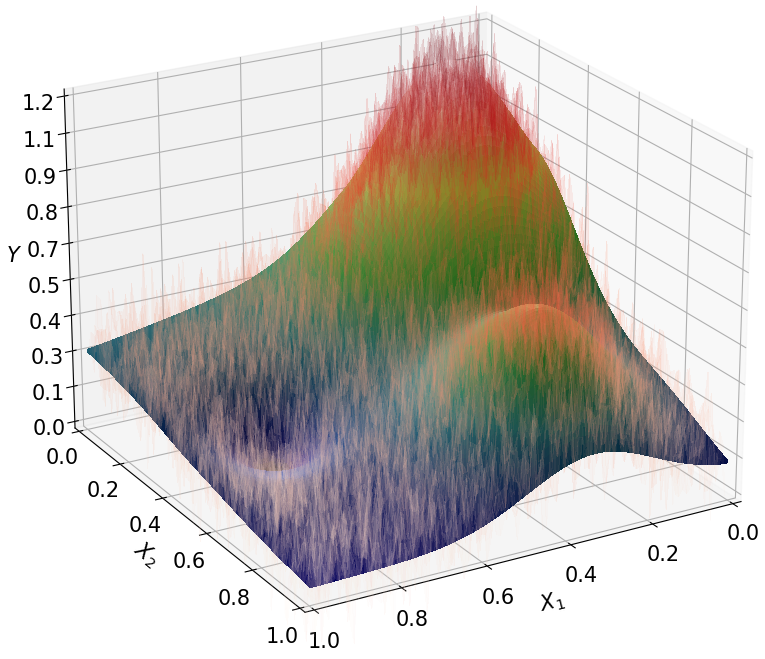
\includegraphics[width=4in, height=3.6in]{Franke_fita.png}}\\
\subfloat[Ridge regression.]{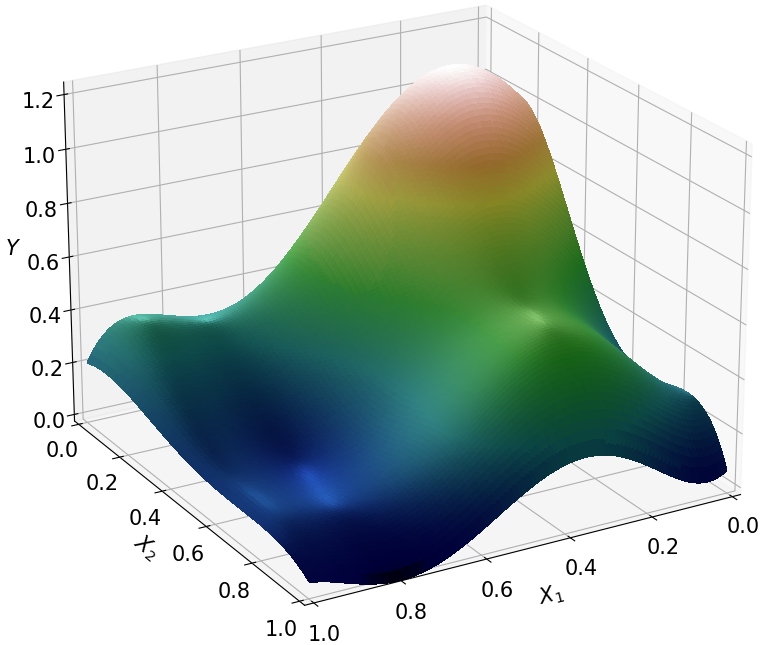
\includegraphics[width=4in, height=3.6in]{Franke_fitb.png}}
\caption{Figure (a) is the Franke's function, which has been generated using 10000 data points  includes an added noise term that follows a normal distribution with an expected value of 0 and a variance of 0.1 (shown in red). Figure (b) is  the results of fitting the function using Ridge regression. The model with the lowest mean squared error (MSE) test from table 1 is used.}
\end{figure}







\begin{figure}[H]
\centerline{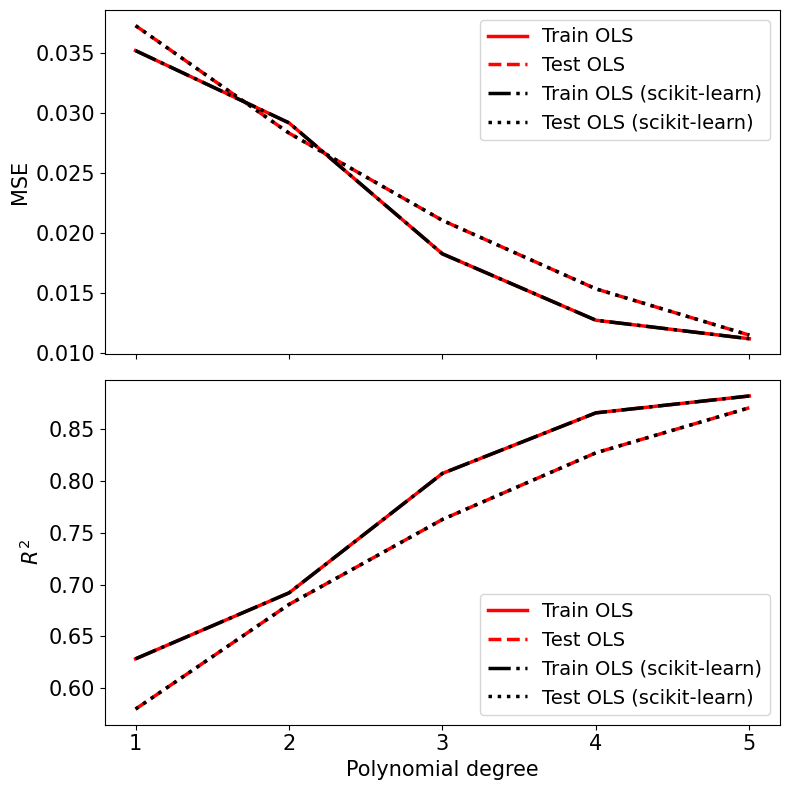
\includegraphics[width=4.2in, height=4.2in]{MSE-R2-OLS.png}}
\caption{Comparing my custom code for ordinary least square regression, which is constructed from 400 data points with a variance of 0.1 and a mean value of 0, to the scikit-learn library, we can see that both yield identical results. When increasing the models complexity this leads to a reduction in mean squared error and the $R^2$ score is improved. }
\label{fig}
\end{figure}

\begin{figure}[H]
\centerline{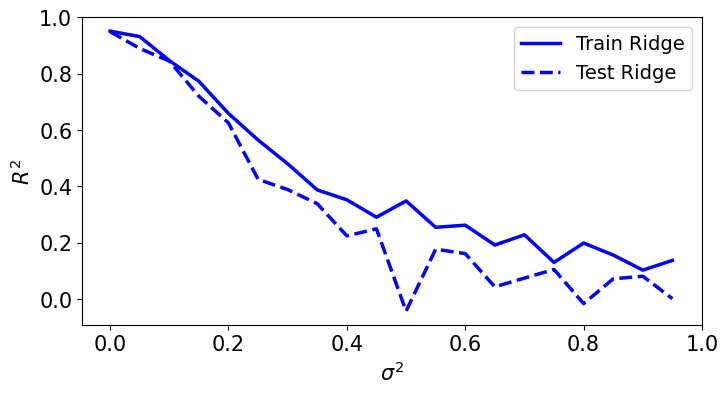
\includegraphics[width=5in, height=2.5in]{Noise-R2.png}}
\caption{The $R^2$ scores for Ridge regression with a hyperparameter of $\lambda=0.001$ are observed. In this analysis, we notice that as the level of noise is introduced to Franke's function, both the training and test fits are affected negatively. Furthermore, it's evident that the training curve provides a better fit compared to the test curve, which is expected as the data becomes increasingly unpredictable. This analysis was conducted using a dataset generated from the Franke's function consisting of 400 data points. }
\label{fig}
\end{figure}



\begin{figure}[H]
\centerline{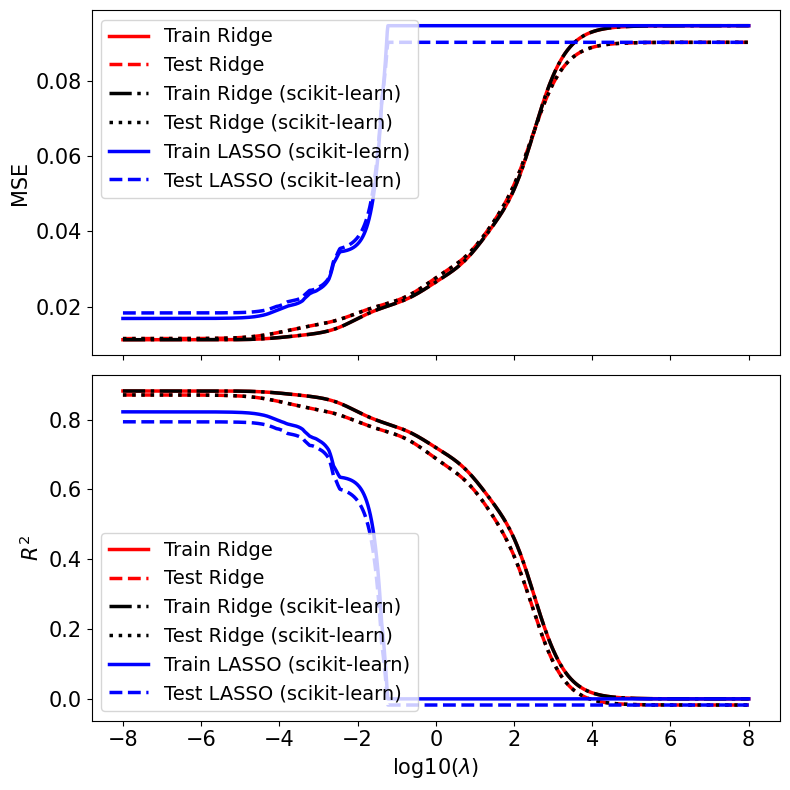
\includegraphics[width=4.4in, height=4.4in]{MSE-R2-Ridge-LASSO.png}}
\caption{When comparing LASSO and Ridge, we observe LASSO regression converges faster to the lowest and highest mean squared errors, and highest $R^2$ scores much faster than Ridge regression. That is; the variance in LASSO aproches zero as $\lambda$ grows larger faster than Ridge. Both Ridge and LASSO regression provide consistent and stable $R^2$ and MSE scores when certain $\lambda$ value is reached. 400 data points are used in this analysis, with a noise term of mean value of 0, variance of 0.1 and a polynomial degree 5. A $\lambda$ value of 0 corresponds to ordinary least squares (OLS) regression. Choosing $\lambda$ values less than 0 results in reduced mean squared error (MSE) and higher $R^2$ scores.}
\label{fig}
\end{figure}


\begin{table}[H]
\caption{Summary of the various regression methods with lowest MSE test values. These findings are obtained from bootstrapping with a polynomial degree of 5. With a small number of data points and low noise, as well as large number of data points, all three regression methods yield similar results. However, when high noise levels are present in the data and number of data points are limited, Ridge and LASSO tend to provide superior predictive performance. } 
\centering 
\begin{tabular}{l l l l l l l} 
\hline\hline 
 n & $\sigma^2$ & $\lambda$ Ridge &MSE Ridge &  $\lambda$ LASSO & MSE LASSO &MSE OLS       \\ [0.5ex] 
\hline 
100    & 0    &$4.3\cdot 10^{-6}$&$7.1\cdot 10^{-3}$ &$3.1\cdot 10^{-11}$ &$1.1\cdot 10^{-2}$&$9.2\cdot 10^{-3}  $ \\
100    & 0.1 &$1.0\cdot 10^{-5} $&$1.4\cdot 10^{-2}$ &$9.3\cdot 10^{-9}$ &$1.6\cdot 10^{-2} $&$2.8\cdot 10^{-2}$ \\
100    & 0 .5&$7.3\cdot 10^{-3}$&$1.6\cdot 10^{-1} $ &$4.5\cdot 10^{-6} $ &$1.7\cdot 10^{-1}$&$2.9\cdot 10^{-1} $ \\ 
400    & 0    &$8.2\cdot 10^{-10}$&$3.1\cdot 10^{-3} $ &$2.3\cdot 10^{-8} $ &$1.3\cdot 10^{-2}$&$3.2\cdot 10^{-3} $ \\
400    & 0.1 &$1.1\cdot 10^{-4}$&$1.4\cdot 10^{-2} $  &$6.5\cdot 10^{-7} $&$2.1\cdot 10^{-2} $&$1.6\cdot 10^{-2} $ \\
400    & 0.5 &$9.0\cdot 10^{-4} $&$1.7\cdot 10^{-1} $ &$6.9\cdot 10^{-9} $ &$1.8\cdot 10^{-1} $&$1.9\cdot 10^{-1}$ \\ 
10000& 0    &$1.6\cdot 10^{-6}$ &$2.0\cdot 10^{-3}$ &$9.3\cdot 10^{-11}$ &$6.9\cdot 10^{-3} $&$2.0\cdot 10^{-3} $ \\
10000& 0.1 &$3.0\cdot 10^{-4} $&$1.3\cdot 10^{-2} $ &$1.5\cdot 10^{-8} $ &$1.8\cdot 10^{-2}$&$1.3\cdot 10^{-2} $ \\
10000& 0.5 &$6.4\cdot 10^{-6}$&$2.6\cdot 10^{-1} $&$9.4\cdot 10^{-9} $&$2.6\cdot 10^{-1} $&$2.6\cdot 10^{-1} $ \\ [1ex] 
\hline\hline
\end{tabular}
\end{table}








\begin{figure}[H]
\centerline{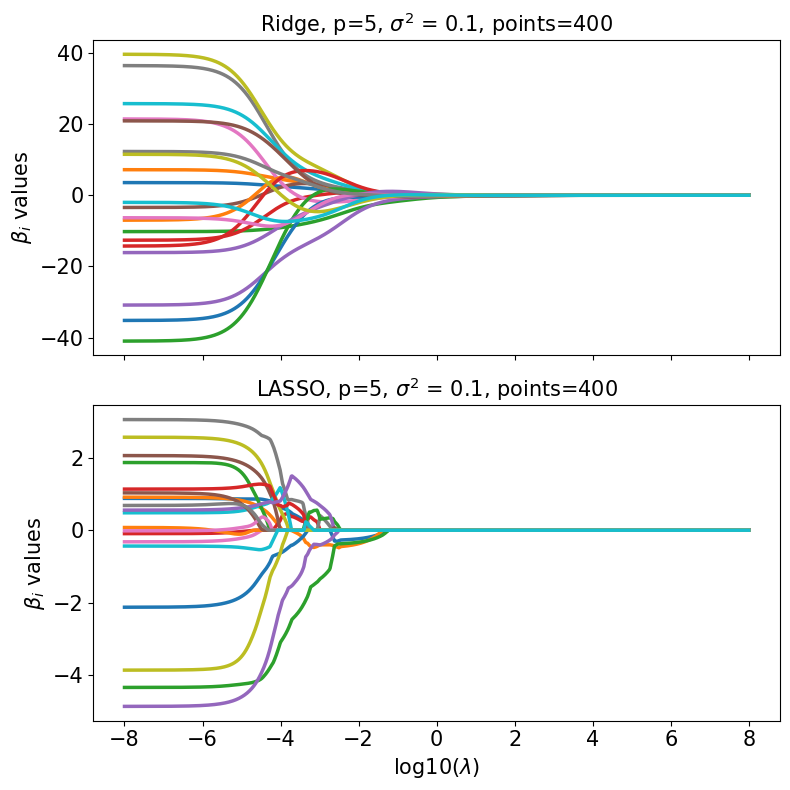
\includegraphics[width=3.9in, height=3.7in]{Ridge-LASSO-beta_values.png}}
\caption{The beta values for both Ridge and LASSO regression as functions of the hyperparameter $\lambda$. Ridge and LASSO regressions have different penalty parameters, and as we can see that the beta values in LASSO regression approaches zero more rapidly compared to the beta values in Ridge regression. These penalty terms contribute to the stabilization of both variance and bias within the models, and therefore leading to better predictive outcomes.}
\label{fig}
\end{figure}

\begin{figure}[H]
\centerline{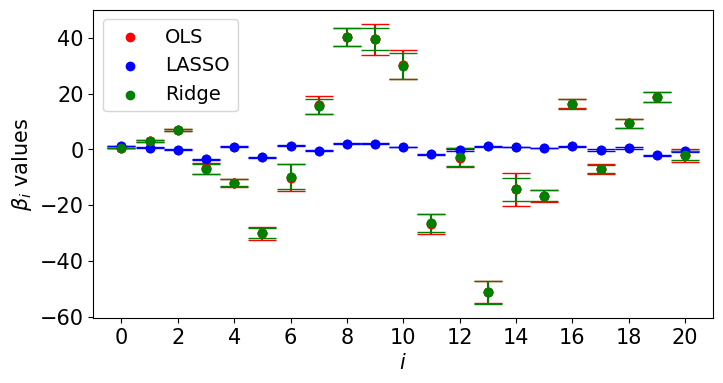
\includegraphics[width=4.8in, height=2.3in]{Error_bar-beta_values.png}}
\caption{Confidence intervals in this figure are computed with $\overline{\beta}_i \pm 1.96 \cdot \sigma_{\beta_i}$for beta values of the different regression methods in this project. These values are derived from 100 bootstraps iterations, of 1000 $\lambda$ values ranging from $10^{-11}$ to 0. The beta values are computed for a polynomial of fifth order, from a dataset generated using Franke's function, consisting of 1000 data points with a variance of 0.1 and 0 mean. Many of the LASSO regression's beta values, obtained through scikit-learn, are excactly zero, however the beta values of Ridge regression are shrunken to achieve the lowest mean squared errors. The beta values from both Ridge and OLS are similar, this is due to the fact that the methods tries to minimize the loss function. Given the range of $\lambda$ values used it is not surprising that they are similar. Had I used larger and fewer $\lambda$ values, Ridge regression would have substantially shrunk the beta coefficients to find optimal solutions.}
\label{fig}
\end{figure}

\begin{figure}[H]
\centerline{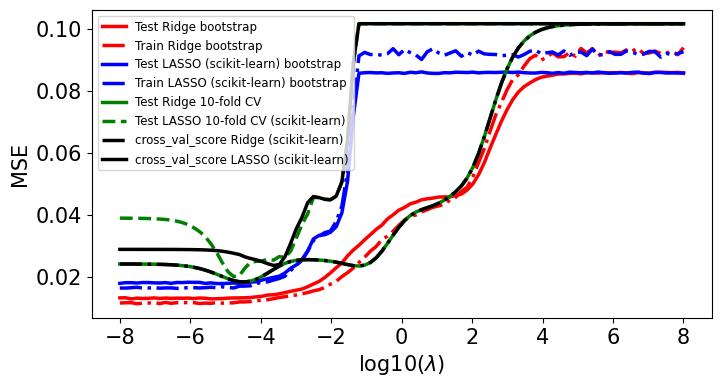
\includegraphics[width=4.8in, height=2.3in]{Ridge_LASSO-comparison.png}}
\caption{These results are similar to those in Figure 3. In LASSO regression, beta values experience substantial shrinkage as $\lambda$ decreases,converging to a consistent MSE values in comparison to Ridge. However, for OLS, both MSE test and MSE train do not converge to a stable values. }
\label{fig}
\end{figure}

\begin{figure}[H]
\centerline{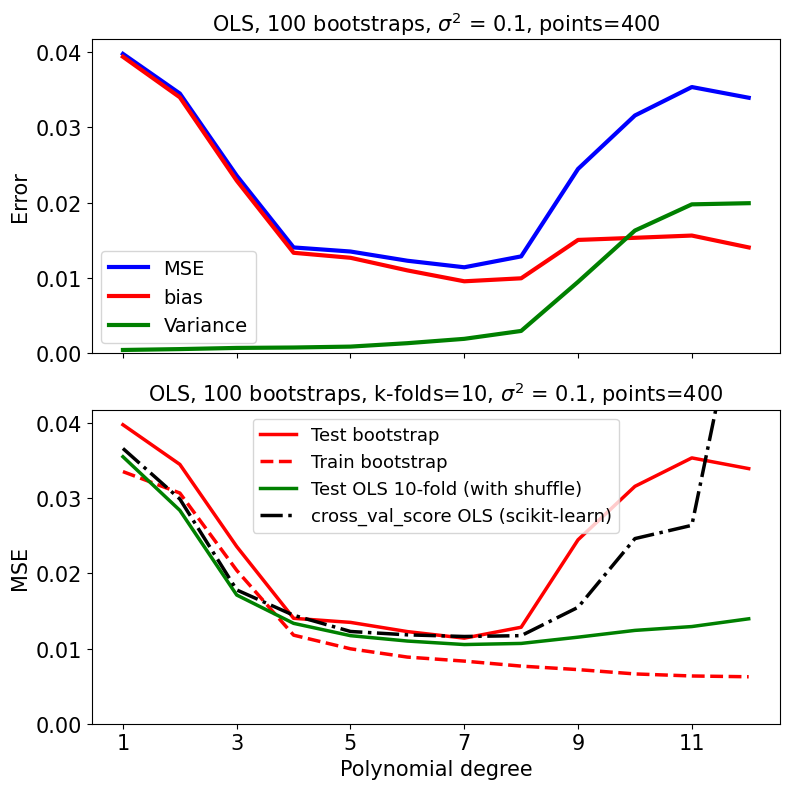
\includegraphics[width=4.8in, height=4.8in]{Bias_variance_tradeoff-MSE.png}}
\caption{Errors, bias, and variance of OLS as functions of polynomial degree, computed from bootstrapping. As $\lambda$ increases, the variance error increases also. On the other hand, the bias error decreases as the model's complexity grows. The bias-variance trade-off lies in balancing both the variance and bias errors when they are minimized, resulting in the lowest MSE. The predicted MSE approximately agrees with the 10-fold CV.}
\label{fig}
\end{figure}









\subsection{Terrain data}

\begin{figure}[H]
\subfloat[Some Norwegian terrain.]{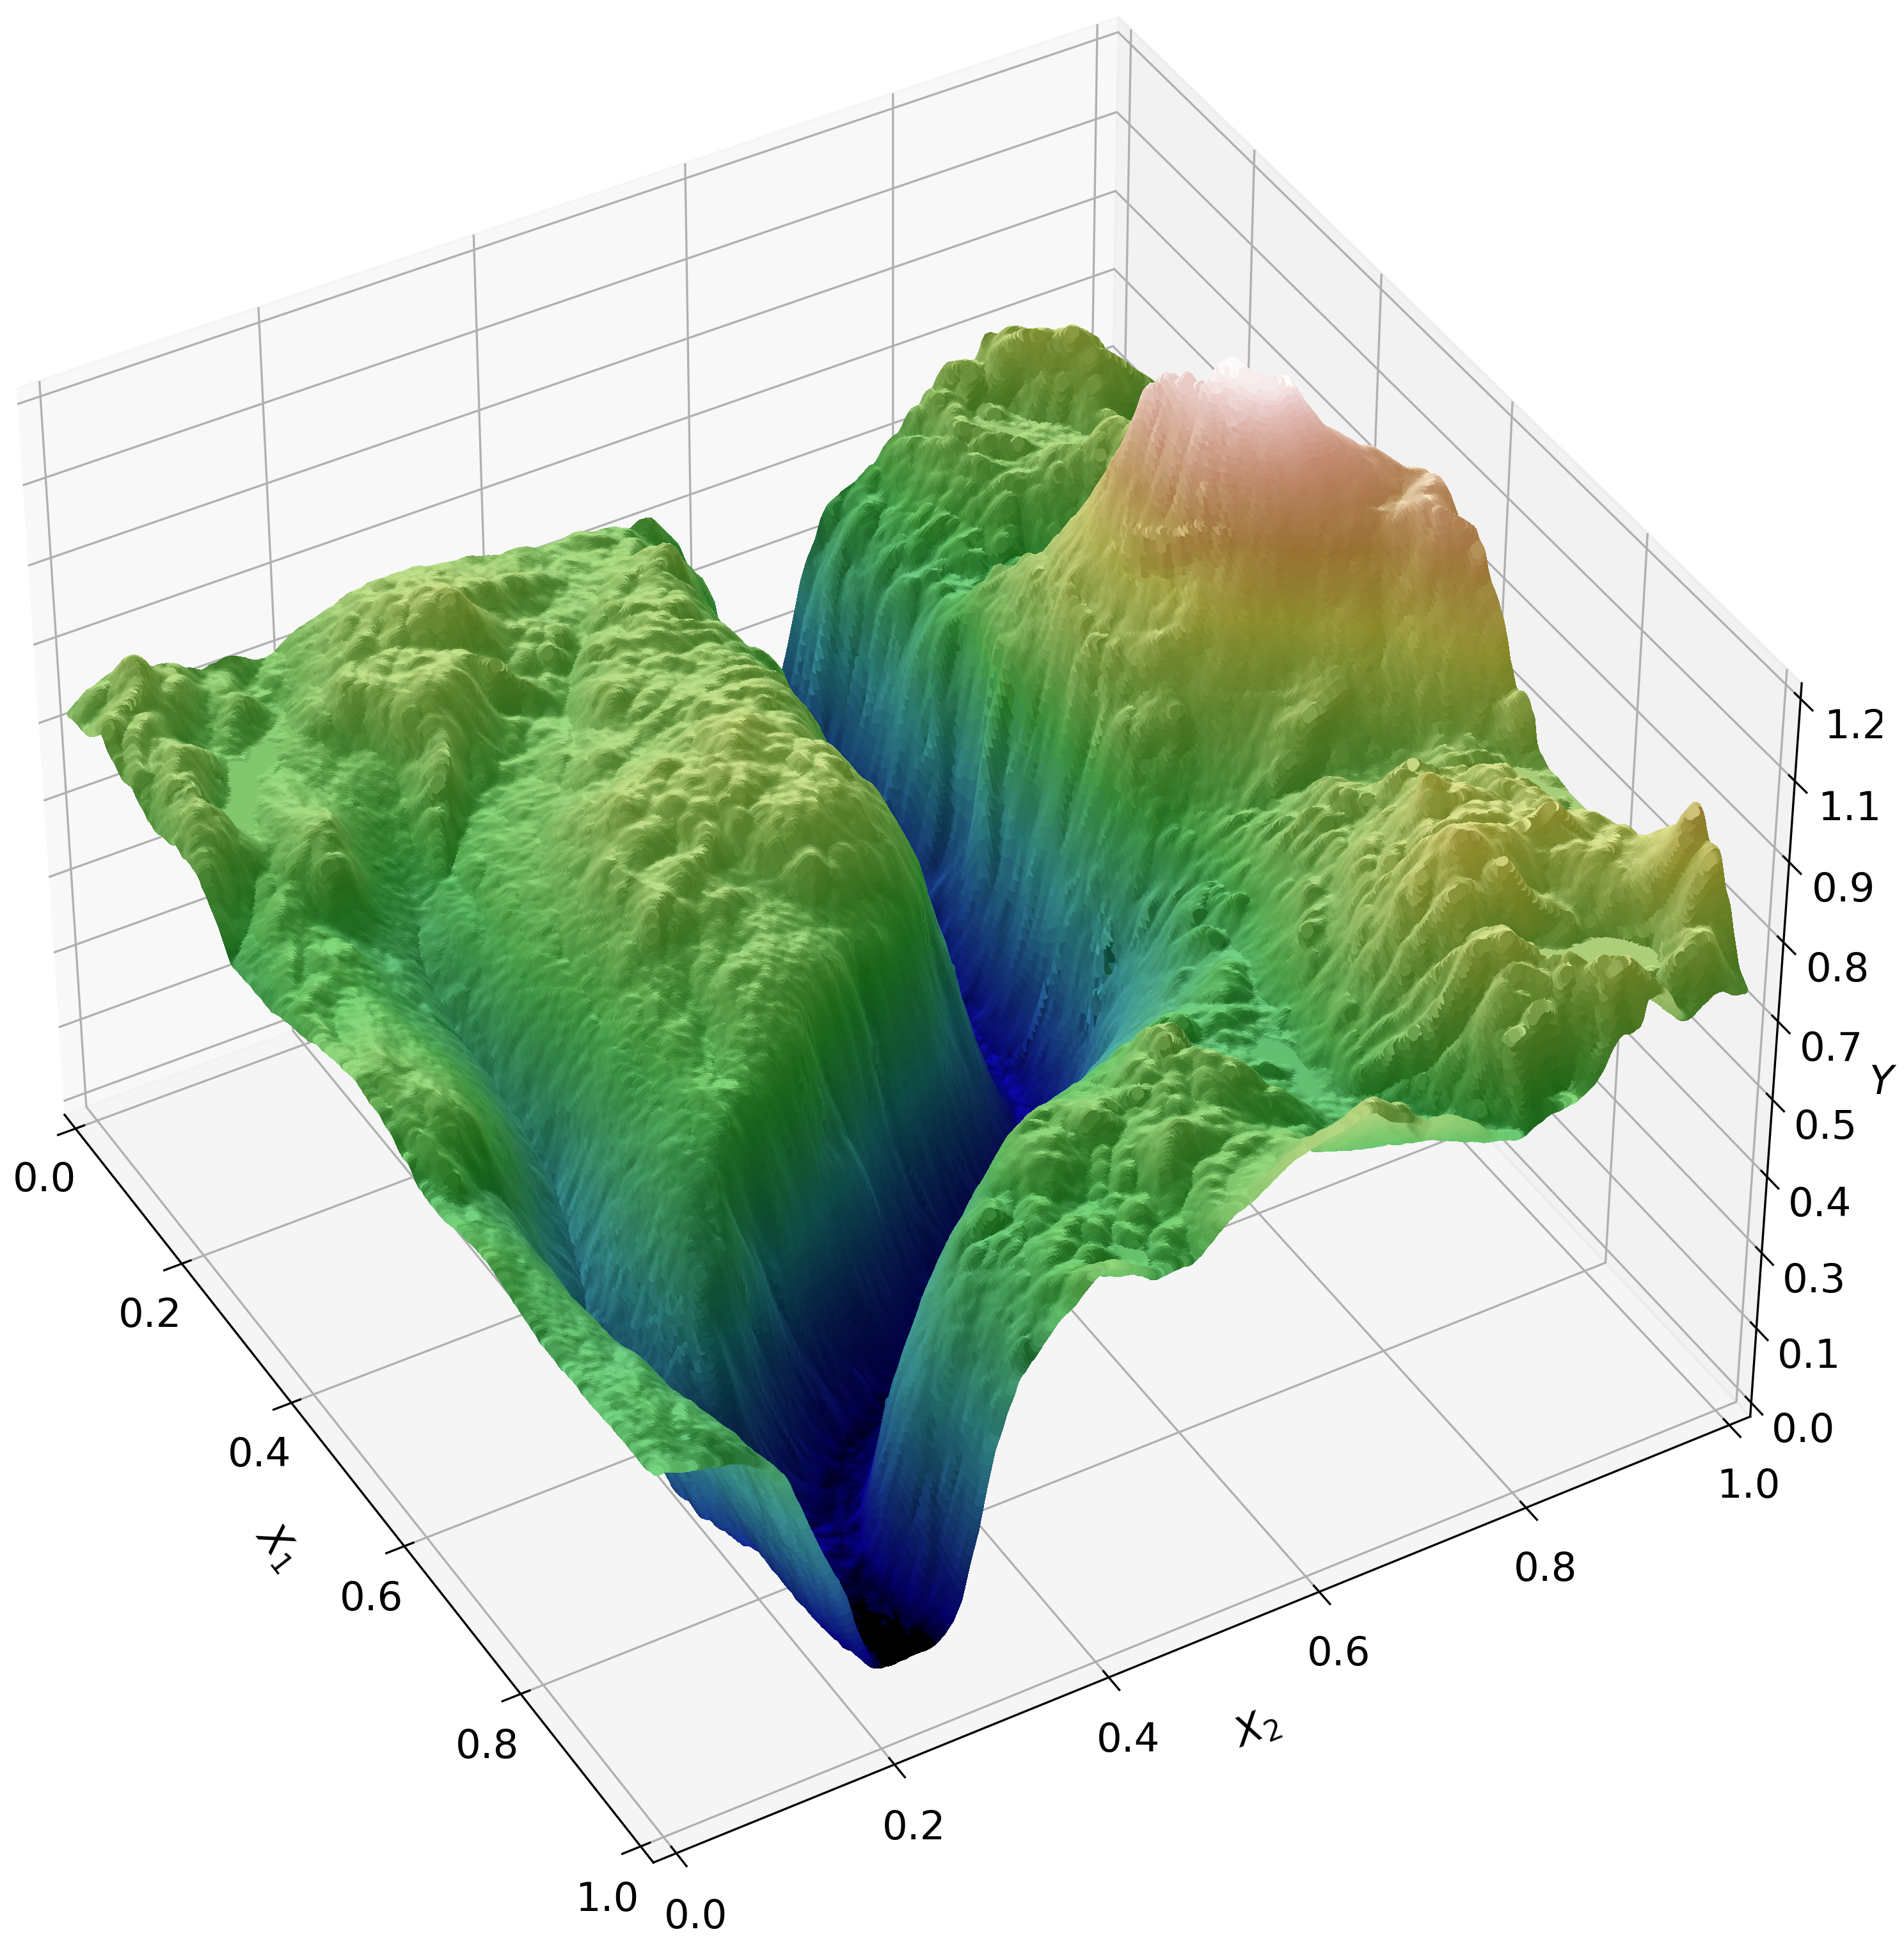
\includegraphics[width=4in, height=3.6in]{Terrain_fita.png}}\\
\subfloat[Ordinary least squares.]{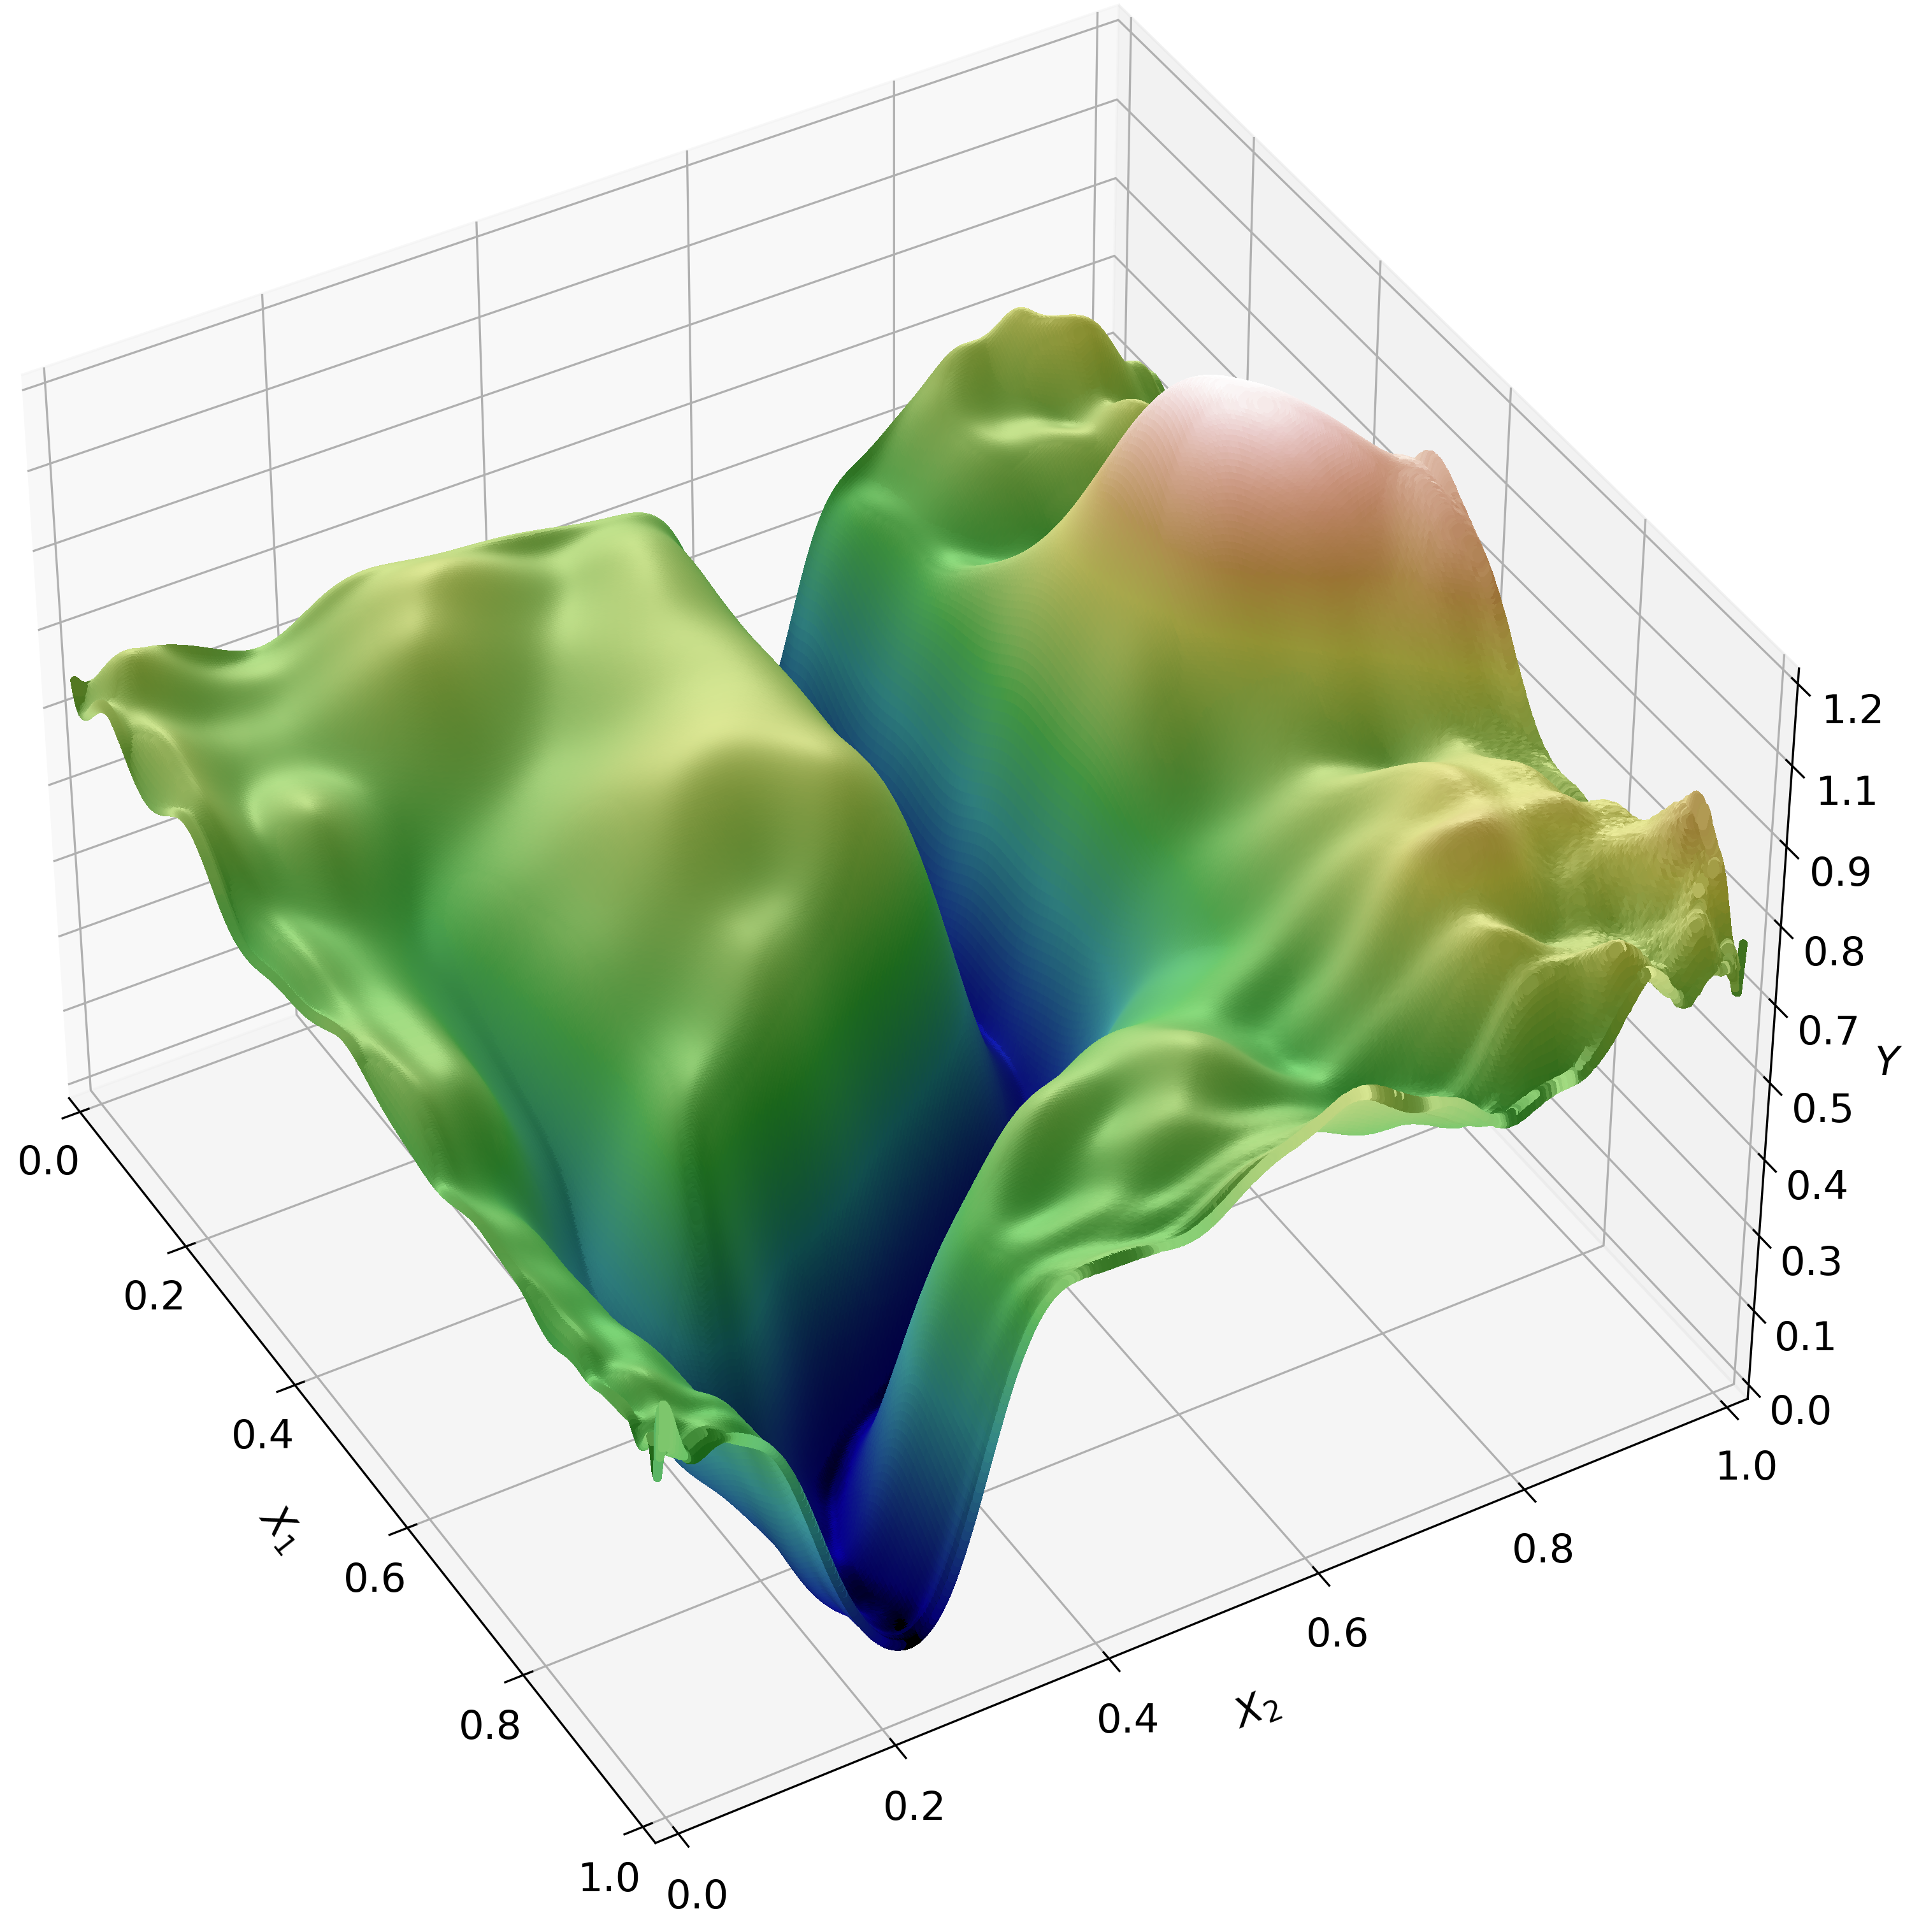
\includegraphics[width=4in, height=3.6in]{Terrain_fitb.png}}
\caption{A section of geographical data, consisting of 160000 data points fig (a). The lowest altitude in this terrain is 193 and highest altitude of 1865. I have normalized the data using the max-min scaling technique, bringing it into alignment with the Franke's function. In Figure (b), you can observe the fitted model, which consisted of 62,500 data points. The mean squared error (MSE) for this ordinary least squares model is $1.5\cdot10^{-4}$.}
\end{figure}




\begin{figure}[H]
\centerline{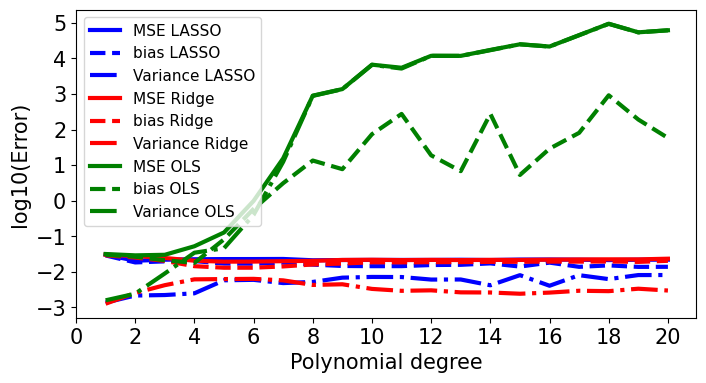
\includegraphics[width=5in, height=2.5in]{best_results-terrain.png}}
\caption{This analysis was conducted on a data set consisting of 100 randomly sampled points from the custom terrain data. Both LASSO and Ridge maintain stable bias and variance, resulting in consistent mean squared errors. In contrast, when it comes to the ordinary least squares method, we observe a similar trend as seen in Franke's function – the errors increase with the rising complexity degrees after achieving the lowest mean squared error. Notice that bias, variance and MSE of Ridge and LASSO er almost a straight line.}
\label{fig}
\end{figure}



\begin{figure}[H]
\centerline{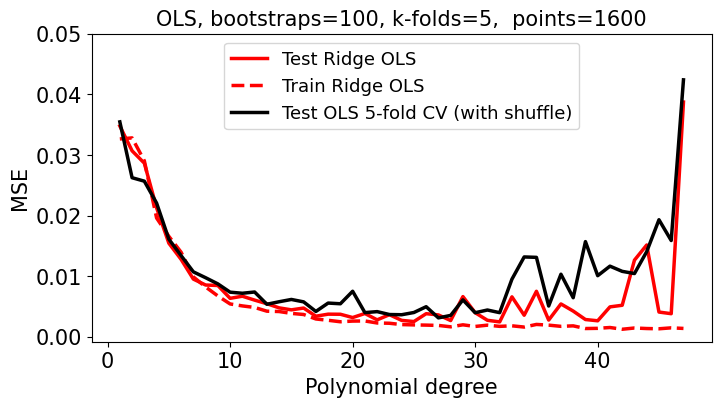
\includegraphics[width=5in, height=2.5in]{Terrain_OLS.png}}
\caption{OLS regression provides good results when there are large number of points used in the model. Just like with the Franke's function, training MSE decreases as the complexity increases and test MSE increases after achieving the tradeoff point. Performance assessment of the model is through k-fold cross validation.}
\label{fig}
\end{figure}


\begin{table}[H]
\caption{The results from the digital terrain data further verifies the results from the Franke's function. Both Ridge and LASSO consistently mitigate overfitting across various complexity degrees, sample sizes and noise levels. Even when OLS achieves its lowest MSE, both LASSO and Ridge outperform it. One important difference from the Franke function analysis is that the optimal $\lambda$ values found in this analysis are significantly smaller.} 
\centering 
\begin{tabular}{l l l l l l} 
\hline\hline 
p  &  $\lambda$ LASSO & MSE LASSO & $\lambda$ Ridge &MSE Ridge&MSE OLS       \\ [0.5ex] 
\hline 
1  &$8.1\cdot 10^{-10}$&$3.0\cdot 10^{-2}$ &$5.5\cdot 10^{-9}$ &$3.0\cdot 10^{-2}$&$3.2\cdot 10^{-2}  $ \\
2  &$7.2\cdot 10^{-4}$&$2.1\cdot 10^{-2}$ &$1.4\cdot 10^{-2}$ &$2.8\cdot 10^{-2}$&$2.9\cdot 10^{-2}  $ \\
3  &$9.7\cdot 10^{-4}$&$2.2\cdot 10^{-2}$ &$6.7\cdot 10^{-3}$ &$2.5\cdot 10^{-2}$&$3.0\cdot 10^{-2}  $ \\
4  &$7.1\cdot 10^{-4}$&$2.3\cdot 10^{-2}$ &$8.2\cdot 10^{-4}$ &$2.1\cdot 10^{-2}$&$5.2\cdot 10^{-2}  $ \\
5  &$1.3\cdot 10^{-4}$&$2.3\cdot 10^{-2}$ &$5.3\cdot 10^{-3}$ &$1.9\cdot 10^{-2}$&$1.3\cdot 10^{-1}  $ \\
6  &$1.9\cdot 10^{-4}$&$2.3\cdot 10^{-2}$ &$8.2\cdot 10^{-3}$ &$1.9\cdot 10^{-2}$&$9.9\cdot 10^{-1}  $ \\
7  &$3.6\cdot 10^{-4}$&$2.3\cdot 10^{-2}$ &$1.9\cdot 10^{-2}$ &$2.0\cdot 10^{-2}$&$1.6\cdot 10^{1}  $ \\
8  &$3.4\cdot 10^{-4}$&$2.1\cdot 10^{-2}$ &$7.2\cdot 10^{-2}$ &$2.0\cdot 10^{-2}$&$9.0\cdot 10^{2}  $ \\
9  &$3.0\cdot 10^{-4}$&$2.1\cdot 10^{-2}$ &$1.0\cdot 10^{-1}$ &$2.2\cdot 10^{-2}$&$1.4\cdot 10^{3}  $ \\
10&$2.4\cdot 10^{-4}$&$2.2\cdot 10^{-2}$ &$2.9\cdot 10^{-1}$ &$2.2\cdot 10^{-2}$&$6.7\cdot 10^{3}  $ \\
11&$3.3\cdot 10^{-4}$&$2.2\cdot 10^{-2}$ &$3.3\cdot 10^{-1}$ &$2.1\cdot 10^{-2}$&$5.5\cdot 10^{3}  $ \\
12&$4.4\cdot 10^{-4}$&$2.2\cdot 10^{-2}$ &$3.9\cdot 10^{-1}$ &$2.2\cdot 10^{-2}$&$1.2\cdot 10^{4}  $ \\
13&$4.9\cdot 10^{-4}$&$2.2\cdot 10^{-2}$ &$6.8\cdot 10^{-1}$ &$2.1\cdot 10^{-2}$&$1.2\cdot 10^{4}  $ \\
14&$6.2\cdot 10^{-4}$&$2.1\cdot 10^{-2}$ &$7.9\cdot 10^{-1}$ &$2.2\cdot 10^{-2}$&$1.7\cdot 10^{4}  $ \\
15&$4.3\cdot 10^{-4}$&$2.2\cdot 10^{-2}$ &$9.5\cdot 10^{-1}$ &$2.2\cdot 10^{-2}$&$2.5\cdot 10^{4}  $ \\
16&$7.1\cdot 10^{-4}$&$2.2\cdot 10^{-2}$ &$9.2\cdot 10^{-1}$ &$2.2\cdot 10^{-2}$&$2.2\cdot 10^{4}  $ \\
17&$4.4\cdot 10^{-4}$&$2.2\cdot 10^{-2}$ &$9.5\cdot 10^{-1}$ &$2.2\cdot 10^{-2}$&$4.5\cdot 10^{4}  $ \\
18&$5.1\cdot 10^{-4}$&$2.1\cdot 10^{-2}$ &$9.7\cdot 10^{-1}$ &$2.2\cdot 10^{-2}$&$9.5\cdot 10^{4}  $ \\
19&$4.1\cdot 10^{-4}$&$2.2\cdot 10^{-2} $&$9.5\cdot 10^{-1} $&$2.2\cdot 10^{-2} $&$5.4\cdot 10^{4} $ \\ 
20&$4.4\cdot 10^{-4}$&$2.2\cdot 10^{-2}$ &$9.6\cdot 10^{-1}$ &$2.3\cdot 10^{-2}$&$6.2\cdot 10^{4}  $ \\ [1ex] 
\hline\hline
\end{tabular}
\end{table}
     


Several of the assumptions made in the theory part are not met when implementing the different methods for the terrain data. One important assumption is that the terrain data doesn't meet the requirement of being independent and identically distributed (i.i.d). Further proof of this is when I performed experiments with models using and not using bootstrapping, and  I obtained significantly better results when without bootstrapping with larger sample size. This was not the case for the Franke function. In the table above, I conducted experiments involving polynomial degrees of 20. Calculations for OLS were not computationally expensive, but for LASSO and Ridge, they consumed a substantial amount of time. This was primarily due to the extensive range of $\lambda$ values considered in the analysis.




\cleardoublepage

\section{Conclusion}

\noindent

\noindent
In this project, I have investigated the advantages and limitations of three different regression methods through various resampling techniques on two different sets of data. The loss function used was mean squared error (MSE), and for the goodness of fit I used persons R-squared. The objective was modeling three-dimensional data by employing feature matrices with varying degrees of polynomial complexity. These methods and techniques have been applied to both the simulated data from the Franke's function with and without added noise and on a section of a actual geographical data representing some terrain in Norway. The effect of hyperparameters on Ridge and LASSO were investigated as well as the effect of noise in the dataset on all regression methods. This was done through many bootstrapping samples, were I calculated means, variance and bias of different models. The models were then assessed through k-fold cross-validation, with iterations of 5 and 10 folds, both with and without shuffle. The scikit-learn library was used to compare my implementation of OLS and Ridge and to get the coefficients for LASSO. \\

\noindent
For the Franke's function and real-world terrain data, all three regression methods exhibit strong predictive capabilities when appropriately configured. In the case of a fixed number of data points and complexity degree, Ordinary Least Squares (OLS) can identify the trade-off point resulting in lowest prediction error on data not used for training. This was not the case for regularized methods since multiple $\lambda$ values can give the same predicted error. The key advantage of Lasso and Ridge lies in their ability to maintain low error, bias, and variance across a wide range of polynomial degrees, data points, and noise levels. Different models used on the Franke's function showed that Ridge and LASSO regression are both more accurate and perform better than OLS when the sample size is small with much noise and low complexities, while for larger sample size and moderate complexity overfitting is reduced and all the methods give similar results.\\

\noindent
Regarding the terrain data, findings closely resembled those of the Franke function. Ridge and LASSO regression consistently yielded strong results when optimal regularization parameters were utilized, regardless of the polynomial degree or sample size, whereas OLS mainly gave satisfactory solutions for larger sample sizes or specific polynomial degrees. Ridge and LASSO, overall, outperformed OLS and provided consistent accuracy. However, determining the optimal regularization parameters proved to be a challenging and time-consuming task. Despite a substantial number of features, I couldn't identify a model that adequately represented the terrain's unique characteristics; instead, the terrain appeared as a smoothed surface in the model. Future research could involve exploring alternative methods that effectively manage complex data, including improved regularization techniques and data scaling based on feature weights. Additionally, incorporating additional features like exponential, logarithmic and Fourier transformations into linear models have potential for better modeling nonlinear data patterns.\\





%---------------------------------------
\cleardoublepage
\addcontentsline{toc}{section}{References}
\bibliography{references}
\begin{thebibliography}{2}

\bibitem{1}
Hastie, Trevor. Tibshirani, Robert. Friedman, Jerome. (2009). The Elements of Statistical Learning Data Mining, Inference, and Prediction. Second Edition. ISBN: 978-0-387-84857-0   

\bibitem{2}
\url{https://compphysics.github.io/MachineLearning/doc/LectureNotes/_build/html/intro.htm} Access date: 8. October 2024

\bibitem{3}
P. Murphy,Kevin. (2022). Probabilistic Machine Learning
An Introduction. ISBN: 9780262046824

\end{thebibliography}
%---------------------------------------

  








\end{document}